\documentclass[a4paper,10pt, twocolumn]{article}
\usepackage[a4paper,top=2cm,bottom=3cm,left=2cm,right=2cm,footskip=0.8cm]{geometry}
\usepackage[utf8]{inputenc}
\usepackage{lipsum}
\usepackage{graphicx}
\usepackage{float}
\usepackage{caption}    % Para personalizar legendas, opcionalrefe
\usepackage{xcolor}
\usepackage{fancyhdr}
\usepackage{helvet}
\usepackage{multicol}
\usepackage{titlesec}     % Para personalizar \section
\usepackage[style=ieee, sorting=nty, language=portuguese]{biblatex}
\definecolor{grayFEI}{HTML}{7F7F7F}
\usepackage{paracol} % no preâmbulo
\usepackage{titlesec}
\usepackage{indentfirst}  % Indenta o primeiro parágrafo
\setlength{\parindent}{2em}  % Aumenta a indentação para 2em (pode ser ajustado
\titlespacing*{\section}{0pt}{*0}{0pt}
\usepackage{ragged2e}
\usepackage{multirow}
\usepackage{array}
\usepackage{booktabs}
\usepackage{tikz}
\usepackage{cuted}
\usetikzlibrary{matrix, positioning, arrows.meta, chains, shapes.geometric, calc, fit, backgrounds}
\usepackage{listings}
\usepackage{adjustbox}
\usepackage{hyperref}
\usepackage{graphicx}
\usepackage{float}
\usepackage{multirow}
\usepackage{tabularx}

\definecolor{codegreen}{rgb}{0,0.6,0}
\definecolor{codegray}{rgb}{0.5,0.5,0.5}
\definecolor{codepurple}{rgb}{0.58,0,0.82}
\definecolor{backcolour}{rgb}{0.95,0.95,0.92}

\lstdefinestyle{mystyle}{
    backgroundcolor=\color{backcolour},   
    commentstyle=\color{codegreen},
    keywordstyle=\color{magenta},
    numberstyle=\tiny\color{codegray},
    stringstyle=\color{codepurple},
    basicstyle=\ttfamily\footnotesize,
    breakatwhitespace=false,         
    breaklines=true,                 
    captionpos=b,                    
    keepspaces=true,                 
    numbers=left,                    
    numbersep=5pt,                  
    showspaces=false,                
    showstringspaces=false,
    showtabs=false,                  
    tabsize=2
}


%-------------------------- ESTILOS NÃO ALTERAR ------------------------------------------------%
% Estilo para legendas de figura e tabela
\captionsetup[figure]{
  labelfont={color=azulFEI, bf, small, sf}, % "Figura" azul, negrito, Arial-like
  textfont={small, sf},                    % Texto da legenda em Arial-like
  font=footnotesize,                       % Tamanho aproximado de 9pt
  labelsep=period,                         % "Figura 1." e não "Figura 1:"
  name=Figura,                             % Tradução para "Figura"
  justification=raggedright,              % Alinhado à esquerda
  singlelinecheck=false                   % Garante alinhamento mesmo em uma linha
}

\captionsetup[table]{
  labelfont={color=azulFEI, bf, small, sf},
  textfont={small, sf},
  font=footnotesize,
  labelsep=period,
  name=Tabela,
  justification=raggedright,
  singlelinecheck=false
}

% Formatação section e subsection
\titleformat{\subsection}
  {\color{grayFEI}\normalfont\fontfamily{phv}\selectfont\itshape\fontsize{10}{12}\selectfont}
  {\thesubsection.}{0.2em}{}
\renewcommand{\thesubsection}{\Alph{subsection}}

\titleformat{\section}
  {\color{azulFEI}\normalfont\fontfamily{phv}\selectfont\bfseries\fontsize{11}{13}\selectfont} % Fonte Helvetica, tamanho 11pt, negrito
  {\thesection.}{0.2em}{}
\renewcommand{\thesection}{\Roman{section}} 
\titlespacing*{\section}
{0pt}{10pt}{0pt}

%Formatação Título
\newcommand{\inovatitle}[1]{%
  \noindent{\fontsize{18}{20}{\helvet{\textbf{\textcolor{azulFEI}{#1}}}}}\vspace{25pt}
}

%Formatação Autores
\newcommand{\autores}[1]{
  \helvet{\fontsize{11}{20}\selectfont\textbf{\textit{#1}}}
}
\newcommand{\orientador}[1]{
  \helvet{\fontsize{11}{20}\selectfont\textbf{\textit{#1}}}
}
\newcommand{\filiacao}[1]{
  \helvet{\fontsize{10}{20}\selectfont{\textit{#1}}}
}
\newcommand{\email}[1]{
  \helvet{\fontsize{10}{20}\selectfont{\textit{#1}}\newline}
}
\newcommand{\resumo}[1]{%
\vspace{15pt}
  \noindent
  {\helvet{\fontsize{12}{20}\selectfont\textbf{\textcolor{azulFEI}{Resumo:}}}} %
  \justifying #1 %
  \newline
}

\newcommand{\keyword}[1]{
  \noindent\helvet{\fontsize{12}{20}\selectfont\textbf{\textcolor{azulFEI}{Palavras-chaves:}}} #1  \vspace{25pt}
}

\renewcommand{\thetable}{\Roman{table}}


% Define a cor azul específica (exemplo: azul FEI)
\definecolor{azulFEI}{HTML}{0070C0} % substitua pelo código que quiser

%Formatação Cabeçalho e rodapé
\setlength{\headsep}{1cm}
\newcommand{\helvet}[1]{{\fontfamily{phv}\selectfont #1}}
\pagestyle{fancy}
\fancyhead{} % limpa cabeçalho
\renewcommand{\headrulewidth}{0.3pt} % ← ATIVA a linha (espessura ajustável)
\setlength\headheight{1.2cm}
\lhead{
\includegraphics[width=4.97cm, height=1cm]{logoinovatcc2.png}}
\rhead{\helvet{2º semestre/2026}}

\fancyfoot{} % limpa rodapé
\lfoot{
  \fontfamily{phv}\fontsize{8}{10}\selectfont
  Anais dos Trabalhos de Conclusão de Curso do Centro Universitário FEI, São Bernardo do Campo – SP\\
  \vspace{-4pt}\rule{\textwidth}{1pt} % ← linha abaixo do texto do rodapé
}
\rfoot{\fontfamily{phv}\fontsize{8}{10}\selectfont \thepage}

%-------------------------------- FIM ESTILOS ---------------------------------------------------%

\addbibresource{referencias.bib}

\begin{document}

\setlength{\columnsep}{20pt}
\twocolumn[
\begin{@twocolumnfalse}

\raggedright

\inovatitle{Tecnologias de Machine Learning para Detecção de Intrusões em Redes de Computadores: Uma Pesquisa Exploratória e Experimental}

\autores{$^1$Lucas Kerr do Amaral, $^2$Marcela Nalesso}

\filiacao{$^1$ Ciência da Computação – FEI}
\filiacao{$^2$ Ciência da Computação – FEI}

\email{$^1$lamaral2002@gmail.com, $^2$marcelanalesso@gmail.com}

\filiacao{Orientador: Prof. Dr. Leonardo Anjoletto Ferreira}
\email{laferreira@fei.edu.br}

\resumo{
	Este trabalho desenvolve um Sistema de Detecção de Intrusão em Redes (NIDS)
	baseado em Aprendizado de Máquina em duas fases. No MVP1, cinco classificadores
	foram comparados na base NSL-KDD, e a \textit{Decision Tree} teve a melhor
	generalização (F1 de 0,835 no \texttt{KDDTest+}) com o menor tempo de inferência. No
	MVP2, foi construído um NIDS conteinerizado que classifica o tráfego em tempo real em
	dois estágios: um \textit{Isolation Forest} não supervisionado e um SVM linear
	supervisionado. O estágio 1 detectou 100\% das varreduras e até 98\% dos
	\textit{beacons} de C2, e o estágio 2 detectou com \textit{recall} de 1,0 o ataque
	volumoso do CIC-IDS-2017, com 0,6\% de falso positivo. O portão de validação
	barrou o envenenamento do treino a partir de 0,10\% do \textit{pool}. Em tráfego real, o sistema
	classificou como benignos 91\% dos alertas de um dia, incluindo os gerados por uma
	queda do link de internet, e classificou como ataque cerca de 1.000 fluxos de uma
	varredura \texttt{nmap} executada no laboratório.
}

\keyword{Detecção de Intrusões, \textit{Machine Learning}, \textit{Isolation Forest}, SVM, Segurança da Informação.}

\end{@twocolumnfalse}
]

\section{Introdução}
A detecção por assinatura não reconhece ataques ainda não catalogados, e o volume
crescente de tráfego amplia a superfície de ataque \cite{Thakkar2021Survey}. O
Aprendizado de Máquina detecta desvios sem regras predefinidas
\cite{Khraisat2019Survey}, mas o tráfego real não tem rótulo e gera muitos falsos
positivos. Este trabalho projeta, implementa e avalia um NIDS que trata os dois
problemas, de um estudo em lote (MVP1) a um sistema em tempo real (MVP2).

\section{Metodologia}
\textbf{MVP1.} Na NSL-KDD, com os 41 atributos padronizados e alvo binário, foram
treinados \textit{Random Forest} (RF), \textit{Decision Tree}
(DT), KNN ($k=5$), Regressão Logística (LR) e SVM linear, com o
\textit{scikit-learn} \cite{scikit2026learn}. A avaliação usou 30\% do
\texttt{KDDTrain+} e o \texttt{KDDTest+}, que tem 17 tipos de ataque ausentes do
treino.

\textbf{MVP2.} O sensor captura passivamente a rede local (Proxmox com
\textit{bridge} em \textit{ageing time} zero), roda em \textit{Docker}
\cite{Merkel2014Docker} e grava em PostgreSQL/TimescaleDB, com painéis no Grafana.
Cada fluxo é descrito por 17 atributos de cabeçalho (volume, tamanho, intervalo
entre pacotes e \textit{flags} TCP). No \textbf{estágio 1}, um \textit{Isolation
Forest} ($c = 0{,}01$) analisa janelas de 10~s, e uma árvore \textit{surrogate}
traduz cada alerta em regra legível. No \textbf{estágio 2}, um SVM linear treinado
com o \textit{golden set} e os vereditos do analista classifica cada alerta como
ataque ou benigno. Antes de entrar em produção, cada novo modelo passa por um portão
de validação contra o \textit{golden set}, que reúne cenários sintéticos (varredura
e \textit{beacon} de C2) e 14.615 fluxos rotulados do CIC-IDS-2017.

\section{Resultados}
\textbf{MVP1.} No \texttt{KDDTest+}, todos os modelos perdem de 16 a 23 pontos de
acurácia em relação à partição retida (Tabela \ref{tab:mvp1}). A DT generaliza
melhor, com \textit{recall} 12 pontos acima do segundo colocado e o menor tempo de
teste. O PCA (23 componentes) piorou a DT (F1 de 0,835 para 0,771), enquanto a
seleção de 18 atributos manteve a acurácia acima de 95\%.

\begin{table}[H]
	\centering
	\footnotesize
	\setlength{\tabcolsep}{3pt}
	\begin{tabular}{lcccccc}
		\toprule
		& \multicolumn{1}{c}{\textbf{Retido}} & \multicolumn{4}{c}{\textbf{\texttt{KDDTest+}}} & \\
		\cmidrule(lr){2-2}\cmidrule(lr){3-6}
		\textbf{Modelo} & \textbf{Acc} & \textbf{Acc} & \textbf{Rec} & \textbf{F1} & \textbf{FPR} & \textbf{Teste (s)} \\
		\midrule
		RF  & 0,999 & 0,765 & 0,608 & 0,747 & 0,028 & 0,037 \\
		DT  & 0,998 & \textbf{0,835} & \textbf{0,732} & \textbf{0,835} & 0,029 & \textbf{0,004} \\
		KNN & 0,996 & 0,769 & 0,612 & 0,751 & 0,025 & 2,567 \\
		LR  & 0,954 & 0,752 & 0,614 & 0,738 & 0,066 & 0,009 \\
		SVM & 0,960 & 0,757 & 0,595 & 0,736 & 0,029 & 7,663 \\
		\bottomrule
	\end{tabular}
	\caption{MVP1: acurácia na partição retida e métricas no \texttt{KDDTest+}.}
	\label{tab:mvp1}
\end{table}

\textbf{MVP2 --- validação dos estágios.} O estágio 1 detectou
\textbf{100\%} das varreduras e de 89\% a 98\% dos \textit{beacons} de C2, com
0,6\% de falso positivo (Tabela \ref{tab:mvp2}): são ataques que geram fluxos raros,
que é o que o \textit{Isolation Forest} isola. A árvore \textit{surrogate} reproduz
99,7\% das suas decisões.

O ataque volumoso do CIC-IDS-2017 é o oposto: milhares de fluxos quase idênticos
formam um aglomerado denso, que um detector de raridade não marca. É o caso que
motiva o estágio 2. Com os \textbf{mesmos 17 atributos}, o SVM o detectou com
\textit{recall} de \textbf{1,0}, F1 de 0,95 e 0,6\% de falso positivo.

No SVM em produção (Figura \ref{fig:svm3d}), a maior parte dos 515 erros (3,7\% de
14.100 fluxos, medidos no próprio treino) são fluxos benignos junto ao hiperplano,
ou seja, falsos positivos, o erro preferível em um IDS.

\begin{figure}[H]
	\centering
	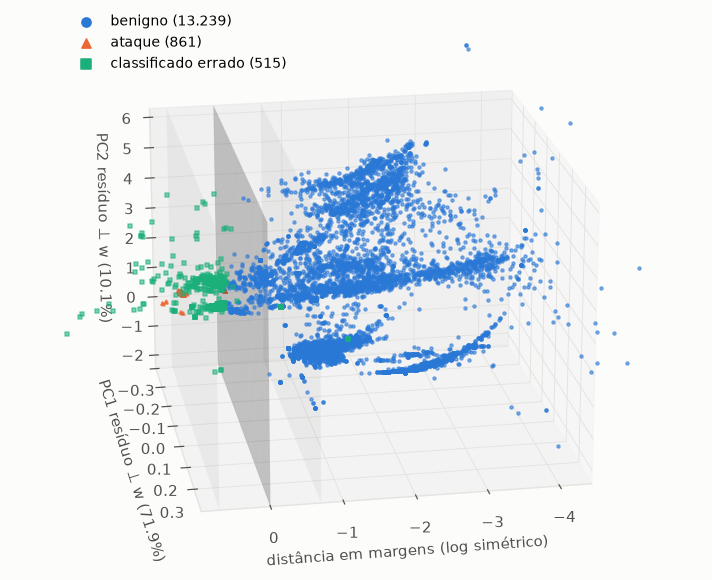
\includegraphics[width=0.9\linewidth]{svm_hiperplano_3d.png}
	\caption{SVM em produção, em base alinhada ao hiperplano (plano cinza).}
	\label{fig:svm3d}
\end{figure}

\begin{table}[H]
	\centering
	\footnotesize
	\setlength{\tabcolsep}{4pt}
	\begin{tabular}{llcc}
		\toprule
		\textbf{Cenário} & \textbf{Base} & \textbf{Estágio 1} & \textbf{Estágio 2} \\
		\midrule
		Varredura         & sintética   & \textbf{1,00} & --- \\
		\textit{Beacon} C2 (1 h) & sintética & 0,89 & --- \\
		\textit{Beacon} C2 (6 h) & sintética & 0,98 & --- \\
		Ataque volumoso   & CIC-IDS-2017 & 0,00 & \textbf{1,00} \\
		\midrule
		\multicolumn{2}{l}{Falso positivo (controle benigno)} & 0,006 & 0,006 \\
		\bottomrule
	\end{tabular}
	\caption{\textit{Recall} por cenário (FPR do estágio 1 na base sintética).}
	\label{tab:mvp2}
\end{table}

\textbf{Resiliência a envenenamento.} Para medir o portão de validação, tráfego de
C2 foi injetado em doses crescentes em um \textit{pool} de 120.000 fluxos (5
sementes). O portão reprovou todo candidato com 0,10\% ou mais de contaminação
(120 fluxos em 120 mil): o atacante não consegue ensinar o detector a ignorá-lo sem
que o retreino seja barrado.

\textbf{MVP2 --- tráfego real.} Sem rótulo em produção, o sistema foi avaliado em
dois eventos de natureza conhecida.

\textit{Anomalia benigna.} O modem do laboratório fica em uma rede própria, ligada à
rede local por um roteador. Ao ser reiniciado, ele derrubou apenas o acesso à
internet, e a rede interna continuou funcionando. O estágio 1 marcou a queda como
anômala (46 alertas às 10h31), e o estágio 2 classificou como benignos todos os 46 e
341 dos 373 alertas do dia (91,4\%), retirando-os do caminho do analista (Figura
\ref{fig:benigna}).

\begin{figure}[H]
	\centering
	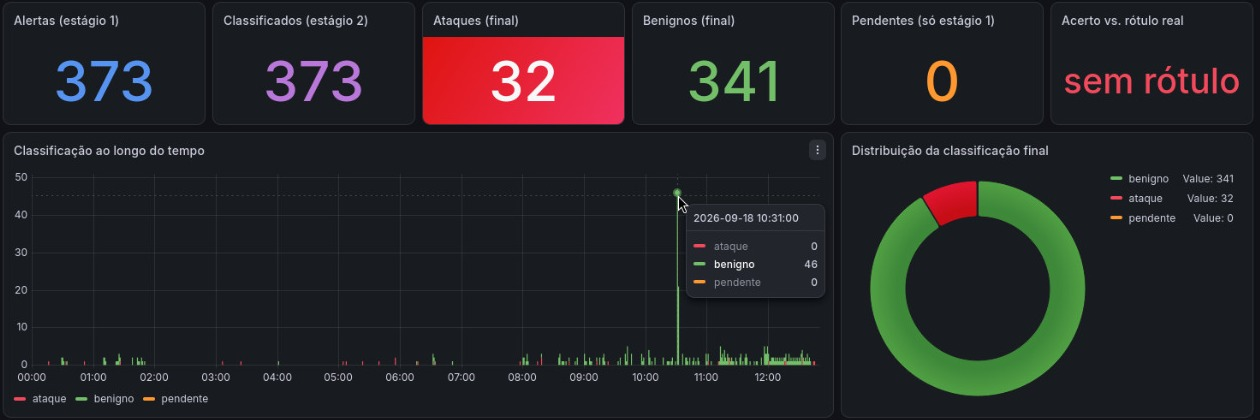
\includegraphics[width=\linewidth]{anomalia_benigna_recorte.jpg}
	\caption{Reinício do modem: alertas classificados como benignos.}
	\label{fig:benigna}
\end{figure}

\textit{Anomalia maligna.} Uma varredura \texttt{nmap} de 1.000 portas, às 12h50, gerou
cerca de 1.000 alertas na mesma janela, e o estágio 2 classificou como ataque todos
menos um (Figura \ref{fig:maligna}). Cada sonda gera um fluxo curto e raro, que o estágio 1
isola.

\begin{figure}[H]
	\centering
	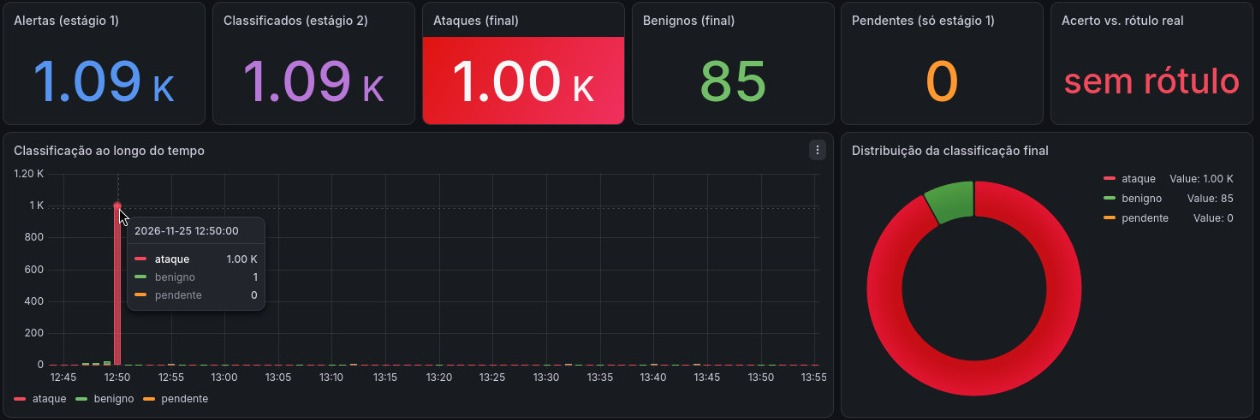
\includegraphics[width=\linewidth]{anomalia_maligna_recorte.jpg}
	\caption{Varredura \texttt{nmap}: alertas classificados como ataque.}
	\label{fig:maligna}
\end{figure}

\section{Conclusão}
A \textit{Decision Tree} foi o melhor classificador em lote. No sistema em tempo real, os dois
estágios se complementam: o \textit{Isolation Forest} sinaliza o que é raro, seja
ataque ou falha de infraestrutura, e o SVM separa um caso do outro. Isso reduziu em
91\% os alertas encaminhados ao analista em um dia de operação e manteve a varredura
de portas classificada como ataque. Como trabalho futuro, a visão agregada por
\textit{host} de origem permitirá que o estágio 1 também encaminhe ao SVM os ataques
volumosos, que hoje só o estágio 2 reconhece.

\section{Referências}
\renewcommand*{\bibfont}{\scriptsize}
\printbibliography[heading=none]

\end{document}
